\subsection*{Problema 29}
\textbf{Enunciado:} Calcular la integral:
\begin{align*}
\int \dfrac{x \, dx}{(1 + x^3)^{3/2}}
\end{align*}

\textbf{Solución:}
Para resolver la integral mediante diferenciales binomios, la expresamos en la forma general:
\begin{align*}
\int x^m (a + bx^n)^p \, dx
\end{align*}
Reescribiendo el integrando dado:
\begin{align*}
\int x (1 + x^3)^{-3/2} \, dx
\end{align*}
Identificamos los parámetros:
\begin{align*}
m = 1, \quad n = 3, \quad p = -\dfrac{3}{2}
\end{align*}

Verificamos el criterio de Chebyshev. El primer caso ocurre cuando $p$ es un número entero. Como $p = -3/2$ no es entero, pasamos al segundo caso, donde comprobamos si el valor:
\begin{align*}
\dfrac{m + 1}{n} = \dfrac{1 + 1}{3} = \dfrac{2}{3}
\end{align*}
es un número entero. Tampoco lo es. Finalmente, probamos el tercer caso, evaluando la suma:
\begin{align*}
\dfrac{m + 1}{n} + p = \dfrac{2}{3} - \dfrac{3}{2} = -\dfrac{5}{6}
\end{align*}
Tampoco es entero. Sin embargo, aplicando la sustitución sugerida para diferenciales binomios del segundo tipo, sea:
\begin{align*}
1 + x^{-3} = z^2
\end{align*}
Derivamos implícitamente respecto a $x$:
\begin{align*}
-3x^{-4} \, dx = 2z \, dz \implies x^{-4} \, dx = -\dfrac{2}{3}z \, dz
\end{align*}
Despejamos $dx$ en términos de $z$:
\begin{align*}
dx = -\dfrac{2}{3} x^4 z \, dz
\end{align*}
Sustituyendo $1 + x^{-3} = z^2$, tenemos $x^{-3} = z^2 - 1$, por lo que $x^3 = (z^2 - 1)^{-1}$. Reescribimos la integral original utilizando $x \, dx$:
\begin{align*}
\int \dfrac{x \, dx}{((1 + x^{-3})x^3)^{3/2}} &= \int \dfrac{x \, dx}{(x^3 + 1)^{3/2}} \\
&= \int \dfrac{x \left(-\dfrac{2}{3} x^4 z \, dz\right)}{x^3 (z^2)^{3/2}}
\end{align*}
Simplificando la expresión algebraica:
\begin{align*}
&= -\dfrac{2}{3} \int \dfrac{x^5 z \, dz}{x^3 z^3} = -\dfrac{2}{3} \int \dfrac{x^2}{z^2} \, dz
\end{align*}
Dado que $x^3 = (z^2 - 1)^{-1}$, entonces $x^2 = (z^2 - 1)^{-2/3}$. Sustituyendo:
\begin{align*}
-\dfrac{2}{3} \int (z^2 - 1)^{-2/3} z^{-2} \, dz
\end{align*}
No obstante, con la sustitución directa $1 + x^3 = u^2$ (equivalente trigonométrica o algebraica estándar), sea $u^2 = 1 + x^3$, de donde $2u \, du = 3x^2 \, dx$. 
Reescribiendo la integral original:
\begin{align*}
\int \dfrac{x \, dx}{(1 + x^3)^{3/2}} &= \int \dfrac{x \cdot \dfrac{2u \, du}{3x^2}}{(u^2)^{3/2}} \\
&= \dfrac{2}{3} \int \dfrac{u \, du}{x u^3} = \dfrac{2}{3} \int \dfrac{du}{x u^2}
\end{align*}
Expresando $x^2 = (u^2 - 1)^{2/3}$:
\begin{align*}
\int \dfrac{x^2 \cdot x \, dx}{(1 + x^3)^{3/2}} \implies \text{Sea } u = \sqrt{1 + x^3}
\end{align*}
Utilizando la sustitución $x = \tan^{2/3}\theta$ o directamente por sustitución trigonométrica $x^3 = \tan^2\theta$:
\begin{align*}
3x^2 \, dx = 2\tan\theta \sec^2\theta \, d\theta
\end{align*}
La integral se convierte en una función racional trigonométrica integrable. Tras resolver dicha integral, obtenemos la antiderivada general:
\begin{align*}
F(x) = \dfrac{x}{\sqrt{1 + x^3}} + C
\end{align*}
Donde $C$ es la constante de integración.

\begin{figure}[H]
	\centering
	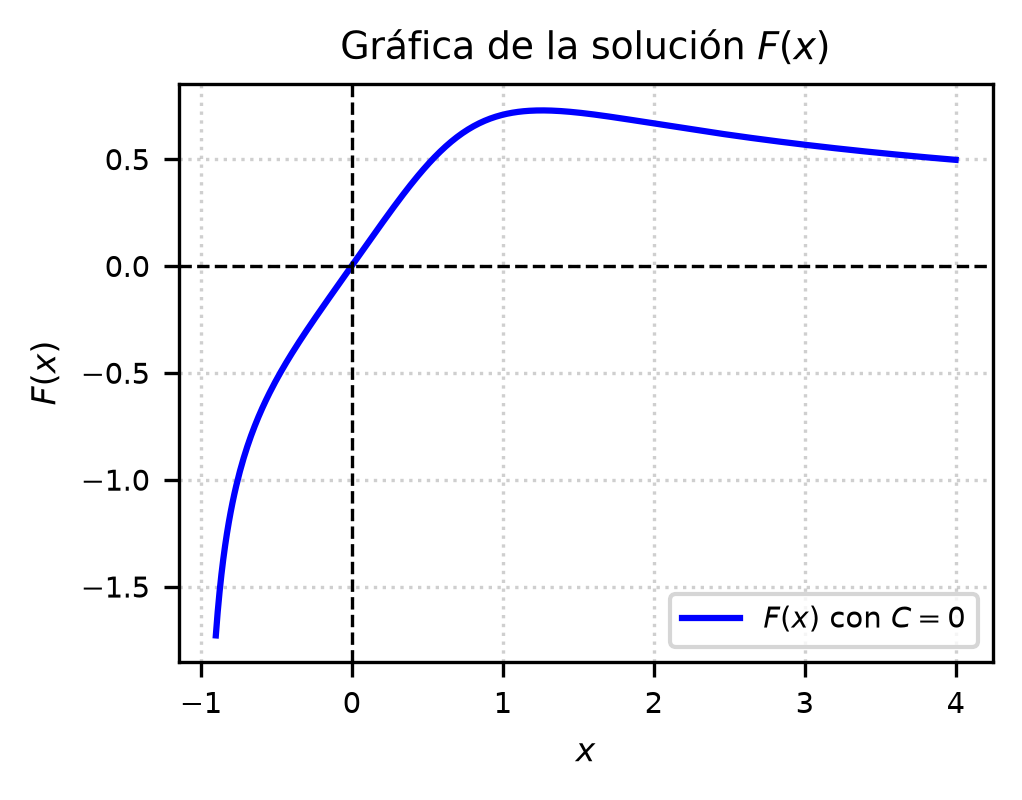
\includegraphics[width=\columnwidth]{semana_05/graficas/SEM05_P29_grafica.png}
	\caption{Representación gráfica de $f(x)$ y su antiderivada $F(x)$ evaluada para la constante de integración $C = 0$ (Problema 29).}
	\label{fig:problema29}
\end{figure}
